\documentclass{exam}
\usepackage{mainExam}

\title{Contrôle : fonction inverse}
\author{Terminale STMG2}
\date{10 Décembre 2024}

\begin{document}
\maketitle

\begin{questions}
\titledquestion{Exercice Type}[7]
Soit $f$ une fonction définie par $f(x) = 3x^2 - 28x - 64/x$.
\begin{parts}
\part[1] Sur quel ensemble cette fonction est-elle définie ?
\part[1] Dériver la fonction sur son ensemble de définition.
\part[2] Montrer que la dérivée que vous venez de calculer vaut, pour tout $x$,
\begin{equation*}
f'(x) = \dfrac{(x-2)(x-4)(6x + 8)}{x^2}
\end{equation*}
\part[3] À l'aide des réponses précédentes, compléter le tableau des variations de $f$ suivant :
\vspace*{0.5cm}
\begin{center}
\begin{tikzpicture}
\tkzTabInit[espcl=2]{$x$/1,Signe de $(x-2)$/1, Signe de $(x - 4)$/1,Signe de $(6x+8)$/1,Signe de $f'(x)$/1,Variations de $f$/2}{$-\infty$,$\dots$,$0$,$\dots$,$\dots$,$+\infty$};
\tkzTabLine{,,,,d,,z,,,,};
\tkzTabLine{,,,,d,,,,z,,};
\tkzTabLine{,,z,,d,,,,,,};
\tkzTabLine{,,z,,d,,z,,z,,};
\tkzTabLine{,,,,d,,,,,,};
\end{tikzpicture}
\end{center}
\end{parts}
\vspace*{1cm}
\titledquestion{Limites de fonctions}[3]
Sur la figure suivante sont représentées trois fonctions ($f$, $g$ et $h$) définies sur $]3;+\infty[$.
\begin{center}
\includegraphics[width=0.9\textwidth]{Figure.png}
\end{center}
\begin{parts}
\part[1,5] Par lecture graphique, donner les valeurs des limites suivantes :
\begin{subparts}
\subpart $\underset{x \to 3^+}{\lim} f(x)$
\subpart $\underset{x \to +\infty}{\lim} f(x)$
\subpart $\underset{x \to 3^+}{\lim} g(x)$
\subpart $\underset{x \to +\infty}{\lim} g(x)$
\subpart $\underset{x \to 3^+}{\lim} h(x)$
\subpart $\underset{x \to +\infty}{\lim} h(x)$
\end{subparts}
\part[1,5] Représenter sur la figure la courbe représentative d'une fonction $p$ définie sur $]3;+\infty[$ et telle que
\begin{equation*}
\begin{cases}
\underset{x \to 3^+}{\lim} p(x) &= +\infty\\ 
\underset{x \to +\infty}{\lim} p(x) &= +\infty 
\end{cases}
\end{equation*} 
\end{parts}

\end{questions}
\end{document}